\documentclass{beamer}
%\usepackage{beamerthemesplit}
\usepackage{beamerthemebars}
%\usepackage[utf8]{inputenc}
\usepackage{graphicx}
\usepackage{german}
\usepackage{url}
\usepackage{color}
\usepackage{listings}
\lstset{
language=[LaTeX]TeX,		%Programmiersprache
extendedchars=true,	%Erweitertes Char-Set
flexiblecolumns=false, 
tabsize=4,
captionpos=b,  %Caption top (t) oder bottom (b)
%stringspaces=false,
float=false,
basicstyle=\footnotesize\ttfamily,		%Courier f"ur Quelltext und Schrift etwas kleiner
%commentstyle=\color{gruen}, %gruene Kommentare
%keywordstyle=\color{blau},  %blaue Keywords
breaklines			%Zeilenumbruch
,numbers=left
,backgroundcolor=\color{lightgray}% Hintergrundfarbe des Listings 
}  
\title{\LaTeX{} f\"ur wissenschaftliche Arbeiten}
\author{Prof. Dr. Antje Gieraths}
\date{\today}

\begin{document}

\frame{\titlepage}
\frame{
\frametitle{Gliederung}
\tableofcontents
}

\section{Ziel}
\frame{
\frametitle{Motivation und Ziel}
\begin{itemize}
\item Eine Alternative zu Quasi-Standard-Textverarbeitungsprogrammen aufzeigen
\item Neugier wecken
\item Sch"onheit und Vorteile von \LaTeX{} zeigen und praktische Hilfen an die Hand geben
\item Live-Demo :-)
\end{itemize}
}

\section{Was ist \LaTeX{}}
\frame{
\frametitle{Was ist \LaTeX{}}
\begin{itemize}
	\item gesprochen "`Lah-Tech"'
	\item Aufsetzend auf \TeX{} von Donald Knuth zum Setzen von Texten und Formeln
	\item Entwickelt mit Setzern und Druckern "`\dots to typeset beautiful (mathematical) books \dots "'
	\item Makropaket mit einfacheren Befehlen von Leslie Lamport
	\item Kein "`what-you-see-is-what-you-get"' (WYSIWYG) - Programm (Word, OpenOffice), sondern Autor gibt logische Gliederung vor und diese wird nach vorgegebenem Layout umgesetzt
\end{itemize}
}
\frame{
\frametitle{Ein kleines Formelbeispiel}
Cosinus Transformation
\begin{eqnarray*}
\widetilde{F}_k & = & \dfrac{1}{N} \sum_{n=0}^{N-1}{f_n \cos \left ( \dfrac{\pi k (n + \frac{1}{2})}{N} \right )}\\
f_n & = & \widetilde{F}_0 + \sum_{k=0}^{N-1}{F_k \cos \left( \dfrac{\pi k (n + \frac{1}{2}}{N} \right )}\\
& & \text{ Symmetrie: } \widetilde{F}_k = - \widetilde{F}_{2N-k}\\
\end{eqnarray*}
Die Alternative hierzu ist der Formeleditor von Word :-) !
}

\section{Vorteile \& Nachteile}
\frame{
\frametitle{Vorteile}
\begin{itemize}
	\item Wenige Befehle f\"ur logische Struktur, keine f\"ur gestalterische Details
	\item Mathematische Formeln werden sehr gut unterst\"utzt
	\item Fu\ss noten, Literaturverzeichnis, Abbildungsverzeichnis,Tabellen werden mit wenig Aufwand sehr gut unterst\"utzt
	\item F\"ur jedes Betriebssystem verf\"ugbar
	\item Dokumente sind klein und gut austauschbar
	\item Ausgabeformat ist PDF oder PS (Postscript)
\end{itemize}
}
\frame{
\frametitle{Vorteile}
\begin{itemize}
	\item Auch und besonders gro\ss e Dokumente (Bachelor-, Master-, Magister- und Doktorarbeiten) werden sehr gut unterst\"utzt und verarbeitet
	\item Speicher- und Resourcenverbrauch ist m\"a\ss ig
	\item Layouts f"ur Briefe, Artikel, Abhandlungen, B"ucher etc. schon vorhanden
\end{itemize}
}
\frame{
\frametitle{Nachteile gegen"uber WYSIWYG}
\begin{itemize}
	\item Man mu\ss{} ein bisschen "`programmieren"' 
	\item Ver\"anderungen an den vorgegebenen Layouts sind nur mit gr\"osserem Aufwand m\"oglich (diese Layouts sind aber sehr durchdacht)
	\item Text, den man in der Eingabedatei eingibt, sieht nicht so aus, wie er schlie\ss lich gedruckt wird
	\item Layout wird "uber Befehle gesteuert
\end{itemize}
}
\section{Tools}
\frame{
\frametitle{Was braucht man und wo bekommt man es her ?}
\begin{itemize}
\item \TeX Live \url{https://tug.org/texlive/}
\item Texteditor, z.b. \TeX Studio \url{https://www.texstudio.org/} 
\item Online Editor Overleaf \url{https://www.overleaf.com/}
\item Vorlage für Bachelorarbeit \url{https://github.com/UniBw-ETTI-2-IoT/LaTeX-Vorlage}
\end{itemize}
}
\section{Der Editor}
\begin{frame}
	\frametitle{\TeX Studio}
	\begin{center}
		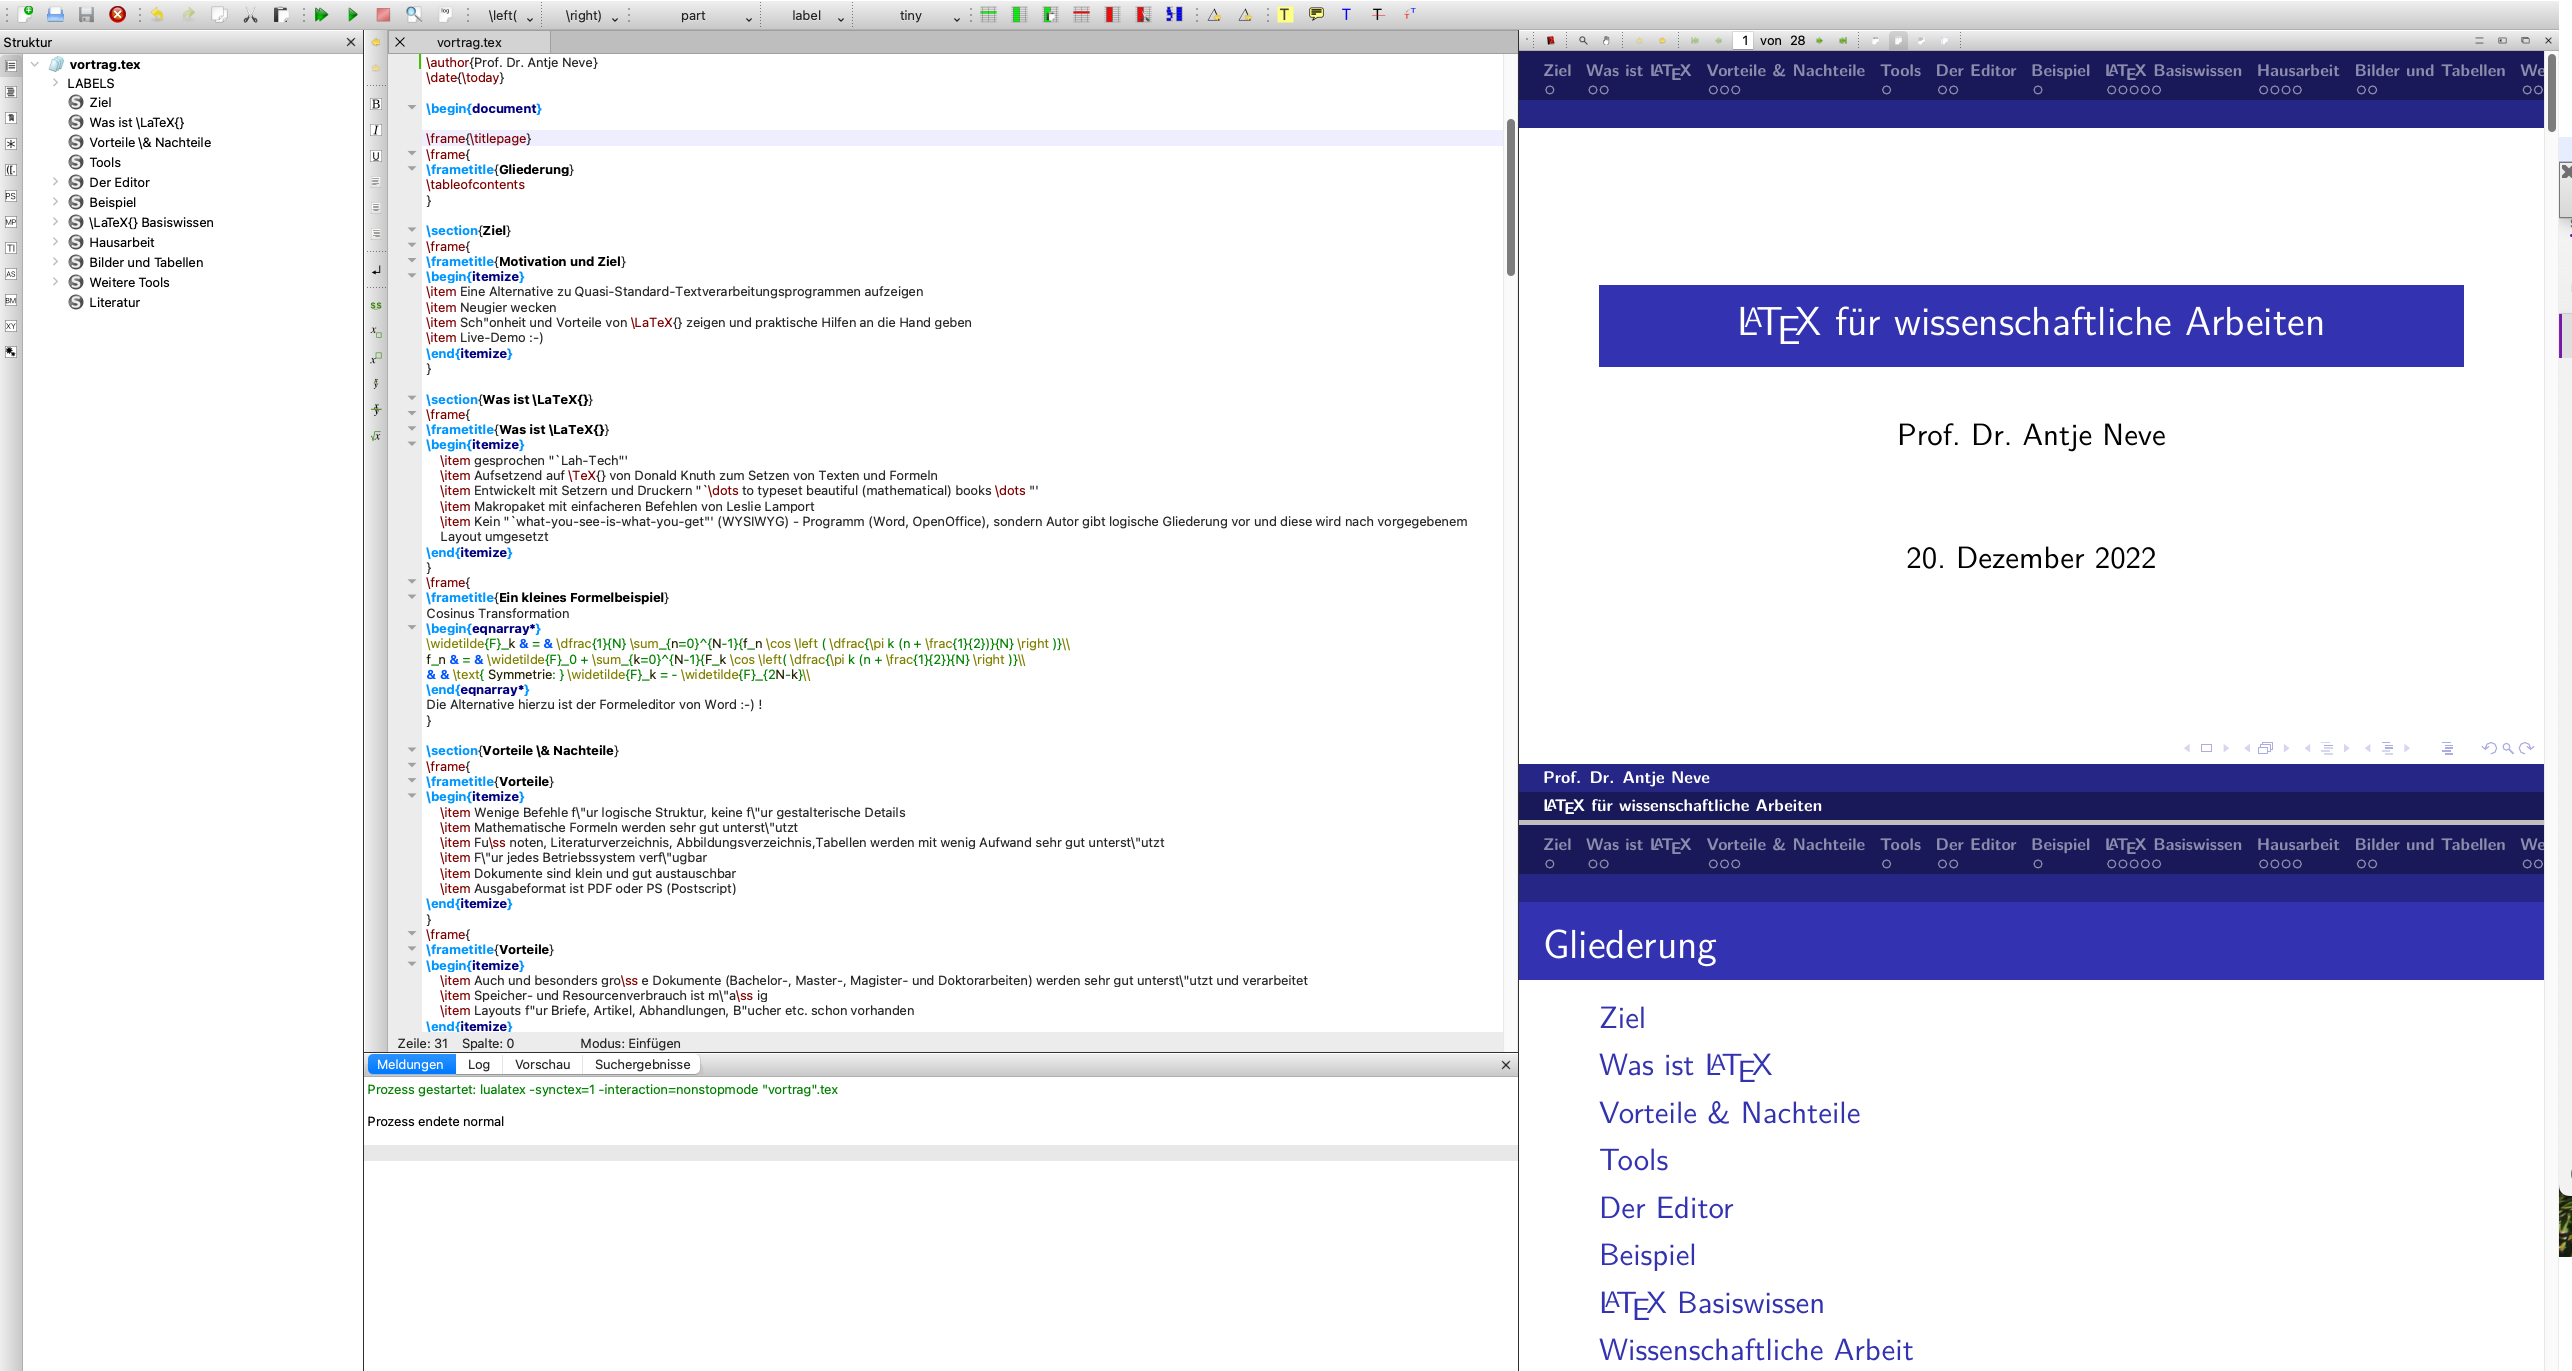
\includegraphics[width=\textwidth]{img/texstudio}
	\end{center}
	
\end{frame}
\begin{frame}
	\frametitle{Overleaf}
	\begin{center}
		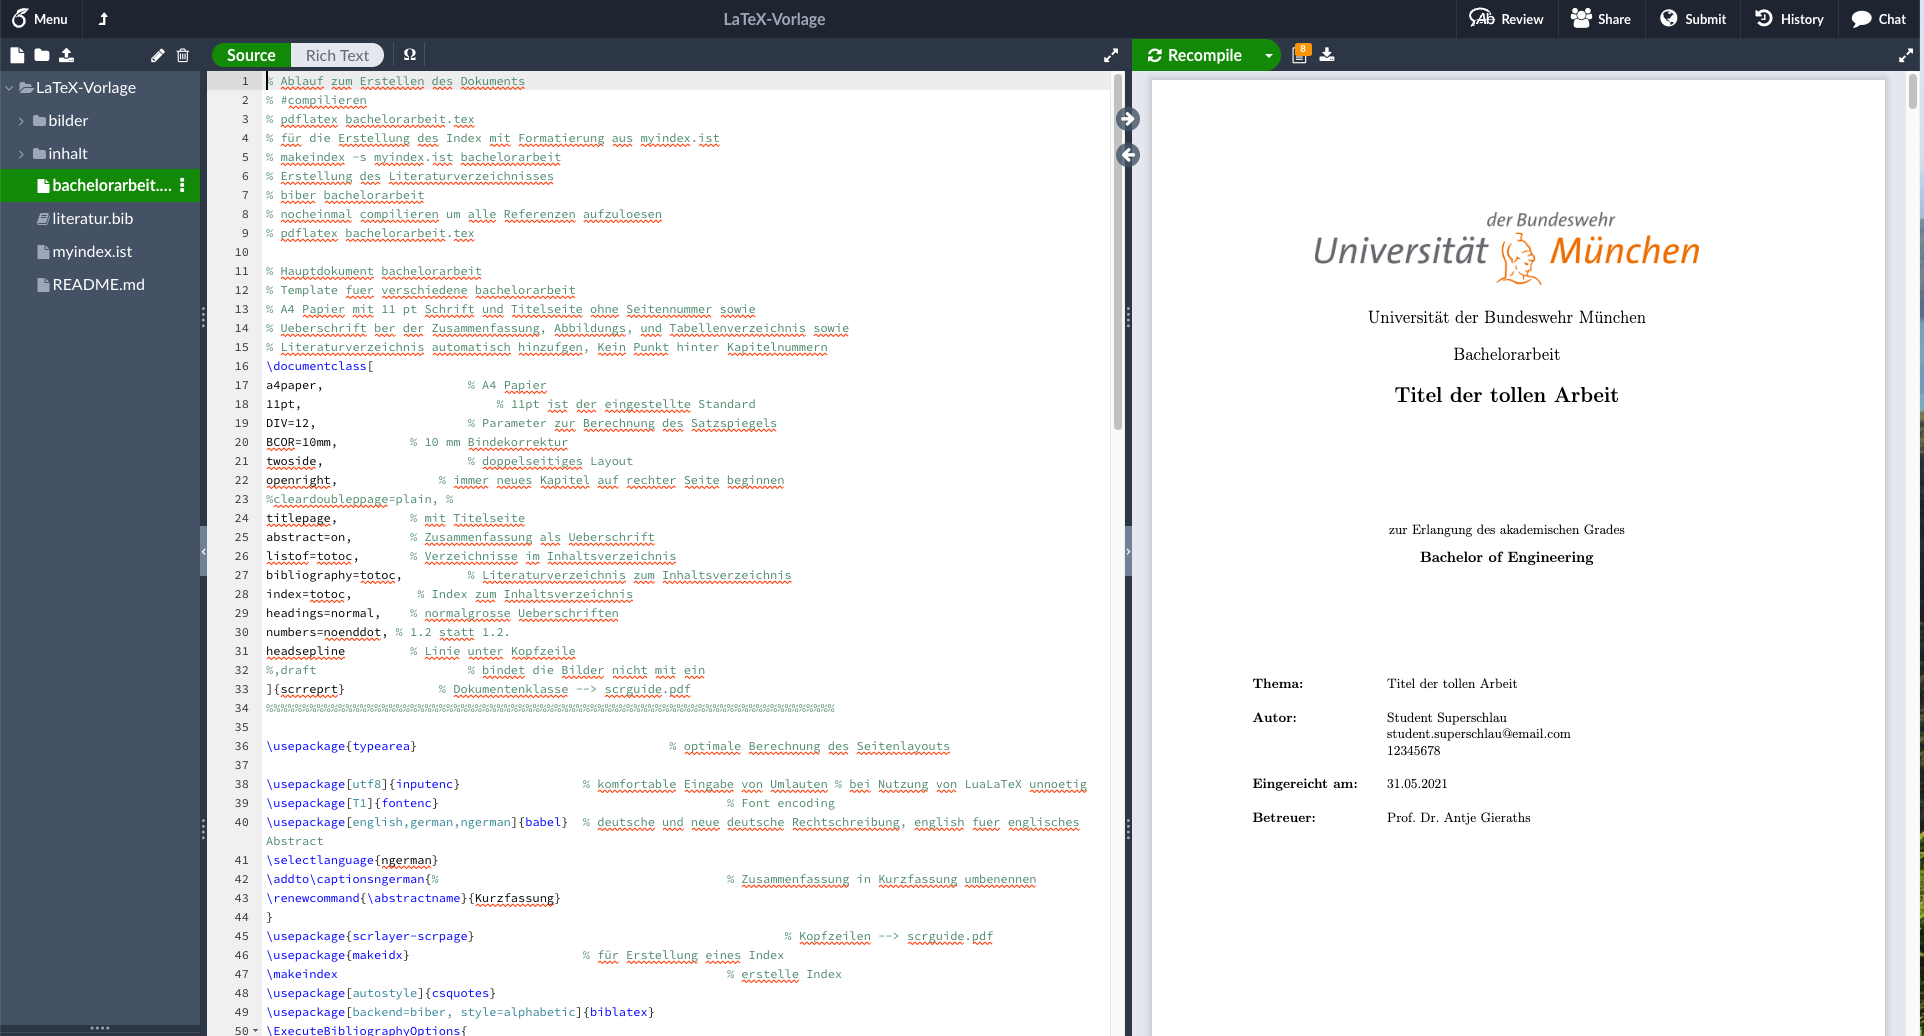
\includegraphics[width=\textwidth]{img/overleaf}
	\end{center}
	
\end{frame}

\section{Beispiel}
\frame[containsverbatim]{
\frametitle{Das erste Beispiel}
\begin{lstlisting}
\documentclass{scrreprt} %Die Dokumentenklasse Report
\begin{document} %Beginn des Eingabetextes
		Mein erstes Beispiel
\end{document} %Ende des Eingabetextes
\end{lstlisting}
Struktur eines \LaTeX{} Befehls:\\
Backslash + Englischer Name des Befehls + Parameter in geschweiften Klammern
\begin{lstlisting}
\documentclass{scrreprt}
\end{lstlisting}
}

\section{\LaTeX{} Basiswissen}
\frame[containsverbatim]{
\frametitle{Basiswissen}
Author, Titel
	\begin{lstlisting}
	\author{M"axchen Muster}
	\title{Meine Diplomarbeit}
	\end{lstlisting}
Gliederung des Textes
	\begin{lstlisting}
	\chapter{Ein Kapitel}
	\section{Ein Abschnitt}
	\subsection{Ein Unterabschnitt}
	\subsubsection{Ein ziemlich tiefer Gliederungspunkt}
	\paragraph{Ein Absatz}
	\subparagraph{Ein Teil eines Absatzes}	
	\end{lstlisting}
}

\frame[containsverbatim]{
\frametitle{Mehr Basiswissen}
Umgebungen, Aufz"ahlungen
\begin{lstlisting}
	\begin{itemize}%Aufzaehlung
		\item Aufzaehlungspunkt
	\end{itemize}
 \begin{enumerate}%nummerierte Aufzaehlung
		\item Nummerierte Aufzaehlung
	\end{enumerate}
\end{lstlisting}
Pakete
	\begin{lstlisting}
	\usepackage[german]{babel} %Sprachpaket
	\usepackage{algorithm2e} %Algorithmen
	\usepackage{hyperref} %Links und Lesezeichen im PDf Dokument
	\end{lstlisting}
}

\frame{
\frametitle{Ein paar \LaTeX{} Grundregeln}
\begin{itemize}
	\item Abs"atze werden durch Leerzeilen getrennt
	\item \LaTeX{} berechnet die Abst"ande zwischen den W"ortern selbst
	\item Mit \% gekennzeichnete Zeilen sind Kommentare
	\item Weitere Sonderzeichen: \&, \#, \$
\end{itemize}
}
\frame[containsverbatim]{
\frametitle{Querverweise und Fu\ss noten}
Querverweise werden automatisch und dynamisch erstellt. 
\begin{lstlisting}
	\section{Ein wichtiger Abschnitt}
	\label{sec:wichtigerAbschnitt}
	Jetzt moechte ich auf den wichtigen Abschnitt verweisen. In \ref{sec:wichtigerAbschnitt} steht dies und jenes. 
\end{lstlisting}
Fu\ss noten gehen ganz leicht und werden automatisch nummeriert.
\begin{lstlisting}
An dieses Wort\footnote{Der Fussnotentext} kommt eine Fussnote.
\end{lstlisting}
}
\frame[containsverbatim]{
\frametitle{Formatierungen \& Gr"o\ss e}
\begin{columns}[t]
\column{0.5\textwidth}
\begin{block}{Formatierung}
\textbf{Fett}\\
\textit{Kursiv} \\
\textsf{serifenlos}\\
\texttt{Schreibmaschine} \\
\textsc{Kapit"alchen}\\
\footnotesize{footnotesize}\\
\large{large}\\
\Large{Large}\\
\Huge{Huge}
\end{block}
\column{0.5\textwidth}
\begin{block}{Befehl}
\begin{lstlisting}
\textbf{Wort}
\textit{Wort}
\textsf{Wort}
\texttt{Wort}
\textsc{Wort}
\footnotesize{Wort}
\large{Wort}
\Large{Wort}
\Huge{Wort}
\end{lstlisting}
\end{block}
\end{columns}
}
\section[Hausarbeit]{Wissenschaftliche Arbeit}
\frame[containsverbatim]{
\frametitle{Wie schreibe ich eine wissenschaftliche Arbeit mit \LaTeX{}}
\begin{enumerate}
	\item Dokumentenklasse heraussuchen, z.B. \lstinline{scrreprt}
	\item evtl. noch ein paar Pakete erg"anzend einf"ugen
	\item Anfangen
\end{enumerate}
\begin{lstlisting}
%Dokumentenklasse Report
\documentclass[a4paper,headsepline, 12pt]{scrreprt}
%eingebundene Pakete
\usepackage[german]{babel} %Sprachpaket
\usepackage{url} %Fuer Internet und Emailadressen, Bsp: \url{antje.gieraths@unibw.de}
\end{lstlisting}
}

\frame[containsverbatim]{
\frametitle{Wie schreibe ich eine wissenschaftliche Arbeit mit \LaTeX{}}
\begin{lstlisting}
%Festlegen des Stils f"ur die Kopfzeilen
\pagestyle{scrheadings}
%Beginn des eigentlichen Dokuments
\begin{document}
%Titelseite:
\titlehead{Universtät der Bundeswehr\\ Fakult"at ETTI}
\subject{Diplomarbeit}
\title{Lauter tolle Sachen "uber ein ganz interessantes Thema}
\author{M"axchen Muster}
\publishers{Erstpr"ufer: Prof. Dr. Schlau \\ Zweitpr"ufer: Prof. Dr. Klug}
\date{FT 2022}
\dedication{Widmung: F"ur meinen Schatz}
\maketitle  %Ende Titelseite/Titelseite erstellen
\end{lstlisting}
}
\frame[containsverbatim]{
\frametitle{Wie schreibe ich eine wissenschaftliche Arbeit mit \LaTeX{}}
\begin{lstlisting}
\tableofcontents %Inhaltsverzeichnis 
\chapter{Einleitung}%1. Kapitel
\label{sec:Einleitung}%Referenzierpunkt
Die Einleitung schreibt man ja meist zum Schluss.
\section{Motivation}
Warum tue ich das hier "uberhaupt ? \\
Hier kommen lauter tolle Gedanken hin. Z.B. in Form einer Auflistung:
\begin{itemize}
	\item Erste Gedanken\footnote{Fu\ss note zu meinem ersten Gedanken}
	\item Zweiter Gedanke
\end{itemize}
\end{lstlisting}
}
\frame[containsverbatim]{
\frametitle{Wie schreibe ich eine wissenschaftliche Arbeit mit \LaTeX{}}
\begin{lstlisting}
Jetzt zitiere ich mal ein Buch \cite{Beispiel:2003} und verweise au\ss erdem auf die Einleitung (\ref{sec:Einleitung}).
%Bibliographie
\bibliographystyle{plain} %Stil der Literaturangabe, alternativ z.B. alpha
\bibliography{literatur}  %Literaturdatenbank bzw.
%Ende des Dokuments
\end{document}\end{lstlisting}
}

\section{Bilder und Tabellen}
\frame[containsverbatim]{
\frametitle{Bilder und Tabellen}
PDF\LaTeX{} oder Lua\LaTeX{} verarbeitet die Bildformate: PDF, JPG, PNG
\begin{lstlisting}
\begin{figure}
	\centering
		\includegraphics[width=1.00\textwidth]{testbild}
	\caption{Eine Bildunterschrift}
	\label{fig:testbild}
\end{figure}
\end{lstlisting}
Tabellen und Bilder k"onnen als Gleitobjekte eingef"ugt werden $\Rightarrow$ optimale Position berechnet \LaTeX{} selbst.

}

\frame[containsverbatim]{
\frametitle{Bilder und Tabellen}
Tabellen gehen so oder mit Excel2\LaTeX{} oder Calc2\LaTeX{} auch bequemer.
\begin{lstlisting}
\begin{table}
	\centering
		\begin{tabular}{l|c|r}
		Spalte 1 & Spalte 2 & Spalte 3 \\
			\hline
			Eintrag 1 & Eintrag 2 & Eintrag 3 \\
		\end{tabular}
	\caption{Eine Tabelle}
	\label{tab:EineTabelle}
\end{table}
\end{lstlisting}
\begin{table}
	\centering
		\begin{tabular}{l|c|r}
		Spalte 1 & Spalte 2 & Spalte 3 \\
			\hline
			Eintrag 1 & Eintrag 2 & Eintrag 3 \\
		\end{tabular}
	\caption{Eine Tabelle}
	\label{tab:EineTabelle}
\end{table}

}


\section{Weitere Tools}
\frame{
\frametitle{Was gibt's noch ?}
\begin{itemize}
\item Makeindex f"ur automatisches Indizieren und die Erstellung von Abk"urzungsverzeichnissen, Indizes, Glossaren etc.
\item Biber f"ur das komfortable Erstellen von Literaturverzeichnissen
\item \dots sind beide bei \TeX live sowie Overleaf dabei
\end{itemize}
}

\frame[containsverbatim]{
\frametitle{Ein Beispiel f"ur Bib\TeX}
\begin{itemize}
	\item Bib\TeX verwaltet gro\ss e Literaturdatenbanken
	\item Eintr"age sehen wie folgt aus
	\item Es gibt sch"one Oberfl"achen zum Eingeben, z.B. JabRef
	\item \url{https://www.jabref.org/}
\end{itemize}
\begin{lstlisting}
@BOOK{Beispiel:2003,
    Address        = {G"ottingen},
    Author         = {Wurst, Hans},
    Editor         = {Pingelig, Franz},
    Pages          = {500},
    Publisher      = {{Ein ganz toller Verlag}},
    Title          = {{Mein erstes Buch "uber dies und das}},
    Year           = {2003}
}
\end{lstlisting}
}

\frame{
\frametitle{JabRef - Eine graphische Oberfl"ache f"ur Literaturdatenbanken}
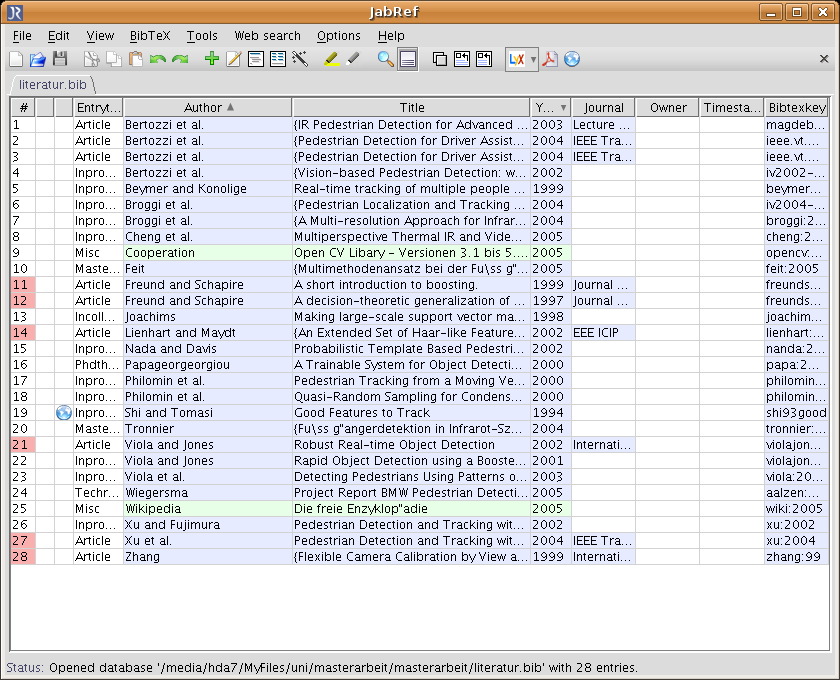
\includegraphics[width=0.7\textwidth]{img/JabRef.png}
}

\section{Literatur}
\frame{
\frametitle{Literatur, Hilfen, Informationsquellen}
\begin{itemize}
	\item Dokumentationen zu den einzelnen Paketen
	\item \url{http://www.dante.de} f"ur \LaTeX{} FAQs, Downloads etc.
	\item Newsgroup: \url{https://groups.google.com/g/de.comp.text.tex?pli=1}
	\item \url{https://en.wikibooks.org/wiki/LaTeX/Mathematics}
	\item \url{https://en.wikibooks.org/wiki/LaTeX/Floats,_Figures_and_Captions}
	\item \url{https://www.overleaf.com/learn}	
	\item \url{https://tex.stackexchange.com/}
\end{itemize}
}
\frame{
\begin{center}
\Huge
(-: Happy \TeX ing ! :-)
\end{center}
}
\end{document}


